% To be \input{}'ed from the various subfolders - do not attempt to compile on
% its own!

\documentclass[10pt]{beamer}
\usepackage[T1]{fontenc}
\usepackage[utf8]{inputenc}

\graphicspath{{}{figures/}{screenshots/}}

\usetheme[progressbar=frametitle]{metropolis}
\usepackage{appendixnumberbeamer}

\usepackage{booktabs}
\usepackage[scale=2]{ccicons}

\usepackage{pgfplots}
\pgfplotsset{compat=1.12}
\usepgfplotslibrary{dateplot}

\usetikzlibrary{calc,fit,patterns}
\usepackage[absolute,overlay]{textpos}

\usepackage{xspace}
\newcommand{\themename}{\textbf{\textsc{metropolis}}\xspace}

\newcommand*{\file}[1]{\texttt{#1}}

\usepackage{xcolor}
\usepackage{listings}
\lstset{columns=fullflexible}
\lstdefinelanguage{EOL}{
morekeywords={delete,import,for,while,in,and,or,self,operation,return,def,var,throw,if,new,else,transaction,abort,
break,breakAll,continue,assert,assertError,not, switch, case, default},
sensitive=true,
morecomment=[l]{//},
morecomment=[l]{--},
morecomment=[s]{/*}{*/},
morecomment=[s]{-*}{*-},
morestring=[b]",
morestring=[b]',
showstringspaces=false
}

\lstnewenvironment{java}{\lstset{language=Java,
		frame=tb,
        tabsize=3,
        morekeywords={implies, in, result},
        basicstyle=\footnotesize,
        keywordstyle=\bfseries,
        ndkeywordstyle=\bfseries,
        commentstyle=\itshape,
		morecomment=[l]{--},
        stringstyle=\ttfamily,
		showspaces=false,
        flexiblecolumns,
        literate={->}{$\to$}{2} {--}{-$\,$-}{2} {<=}{$\le$}{2} {>=}{$\ge$}{2} {<>}{$<\,>$}{3},
        sensitive, extendedchars, texcl}}{}

\lstnewenvironment{ocl}{\lstset{language=[decorative]OCL,
	frame=tb,
	tabsize=3,
	morekeywords={implies,result,flatten,body,init,OrderedSet,Tuple,TupleType,def,attr,oclIsUndefined,oclIsInvalid,OclState,let,in},
	basicstyle=\footnotesize,
	keywordstyle=\bfseries,
	ndkeywordstyle=\bfseries,
	commentstyle=\itshape,
	stringstyle=\ttfamily,
	showspaces=false,
	flexiblecolumns,
	literate={->}{$\to$}{2} {--}{-$\,$-}{2} {<=}{$\le$}{2} {>=}{$\ge$}{2} {<>}{$<\,>$}{3},
	sensitive, extendedchars, texcl}}{}


\lstdefinelanguage{gremlin}{
morekeywords={as,def,fill,filter,groupCount,has,idx,inE,inV,is,label,length,match,outE,outV,v,values},
sensitive=true,
morecomment=[l]{//}
}

% "page cs" coordinate system
% From http://tex.stackexchange.com/questions/89588/
%
% Defining a new coordinate system for the page:
%
% --------------------------
% |(-1,1)    (0,1)    (1,1)|
% |                        |
% |(-1,0)    (0,0)    (1,0)|
% |                        |
% |(-1,-1)   (0,-1)  (1,-1)|
% --------------------------
\makeatletter
\def\parsecomma#1,#2\endparsecomma{\def\page@x{#1}\def\page@y{#2}}
\tikzdeclarecoordinatesystem{page}{
    \parsecomma#1\endparsecomma
    \pgfpointanchor{current page}{north east}
    % Save the upper right corner
    \pgf@xc=\pgf@x%
    \pgf@yc=\pgf@y%
    % save the lower left corner
    \pgfpointanchor{current page}{south west}
    \pgf@xb=\pgf@x%
    \pgf@yb=\pgf@y%
    % Transform to the correct placement
    \pgfmathparse{(\pgf@xc-\pgf@xb)/2.*\page@x+(\pgf@xc+\pgf@xb)/2.}
    \expandafter\pgf@x\expandafter=\pgfmathresult pt
    \pgfmathparse{(\pgf@yc-\pgf@yb)/2.*\page@y+(\pgf@yc+\pgf@yb)/2.}
    \expandafter\pgf@y\expandafter=\pgfmathresult pt
}
\makeatother
% Draws a grid for easier referencing of page cs values
\newcommand{\printtikzpagegrid}{
  \tiny
  \begin{tikzpicture}[overlay,remember picture,every node/.style={inner sep=.1em,draw=black!20,fill=white}]
    \foreach \x in {0,...,9} {
      \foreach \y in {0,...,9} {
        \node at (page cs:0.\x,0.\y) {};
        \node at (page cs:0.\x,-0.\y) {};
        \node at (page cs:-0.\x,0.\y) {};
        \node at (page cs:-0.\x,-0.\y) {};
      }
    }
    \node at (page cs:0,0) {0,0};
    \node at (page cs:0.5,0.5) {.5,.5};
    \node at (page cs:0.5,-0.5) {.5,-.5};
    \node at (page cs:-0.5,0.5) {-.5,.5};
    \node at (page cs:-0.5,-0.5) {-.5,-.5};
    \node at (page cs:1,1) {1,1};
    \node at (page cs:1,-1) {1,-1};
    \node at (page cs:-1,1) {-1,1};
    \node at (page cs:-1,-1) {-1,-1};
  \end{tikzpicture}
  \normalsize
}

\title{Taming Large Models\\with Hawk and NeoEMF}
%\subtitle{A modern beamer theme}
\date{MoDELS'2018, 14--19 October 2018}
\author{A. García-Domínguez, D. S. Kolovos, K. Barmpis, G. Daniel, G. Sunyé}
%\institute{Center for modern beamer themes}
% \titlegraphic{\hfill\includegraphics[height=1.5cm]{logo.pdf}}


\begin{document}

\maketitle

\pgfset{/metropolis/inner/sectionpage/.cd, none}
\section{Introduction}

\pgfset{/metropolis/inner/sectionpage/.cd, progressbar}
\section{Hawk}

\begin{frame}{Hawk: indexing for fast querying over fragment collections}
  \centering

  \begin{columns}[t]
    \column{.5\textwidth}
    \centering
    \begin{tikzpicture}[remember picture]
      \node (oldapproach) {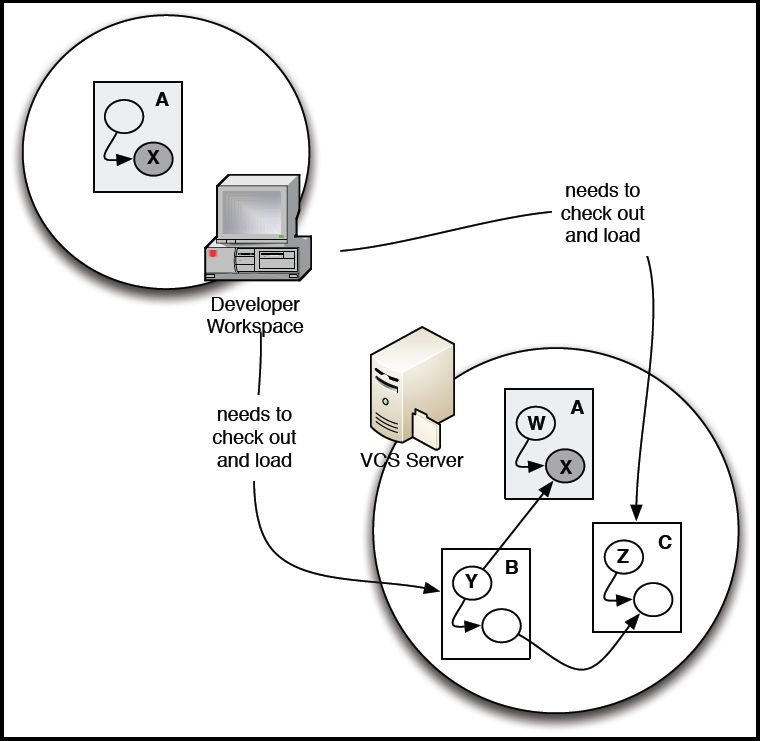
\includegraphics[width=\columnwidth,height=4.15cm,keepaspectratio]{old-approach}};
    \end{tikzpicture}
    \begin{block}{Usual approach}
      \begin{enumerate}
      \item Check out \textbf{all} files from VCS
      \item Load fragments into memory
      \item Run query (might go over all fragments)
      \end{enumerate}
    \end{block}

    \column{.5\textwidth}
    \centering
    \begin{tikzpicture}[remember picture]
      \node (newapproach) {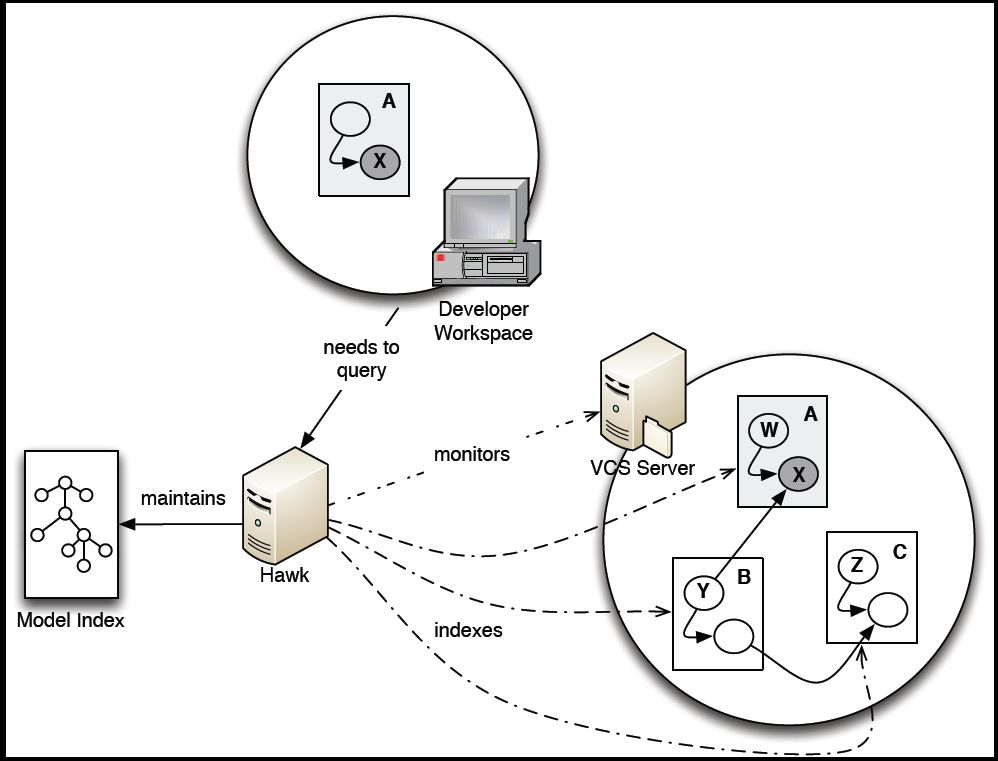
\includegraphics[width=\columnwidth,height=4.15cm,keepaspectratio]{hawk-approach}};
    \end{tikzpicture}
    \begin{block}{With Hawk}
      \begin{enumerate}
      \item Hawk watches VCS, indexes
      \item User queries Hawk over WS
      \item Hawk runs query through NoSQL database efficiently
      \item Hawk replies with result
      \end{enumerate}
    \end{block}

  \end{columns}

  \begin{tikzpicture}[overlay,remember picture]
    \draw[ultra thick,red,->] (oldapproach) -> (newapproach);
  \end{tikzpicture}
\end{frame}

\begin{frame}{Deployment}

  \begin{center}
    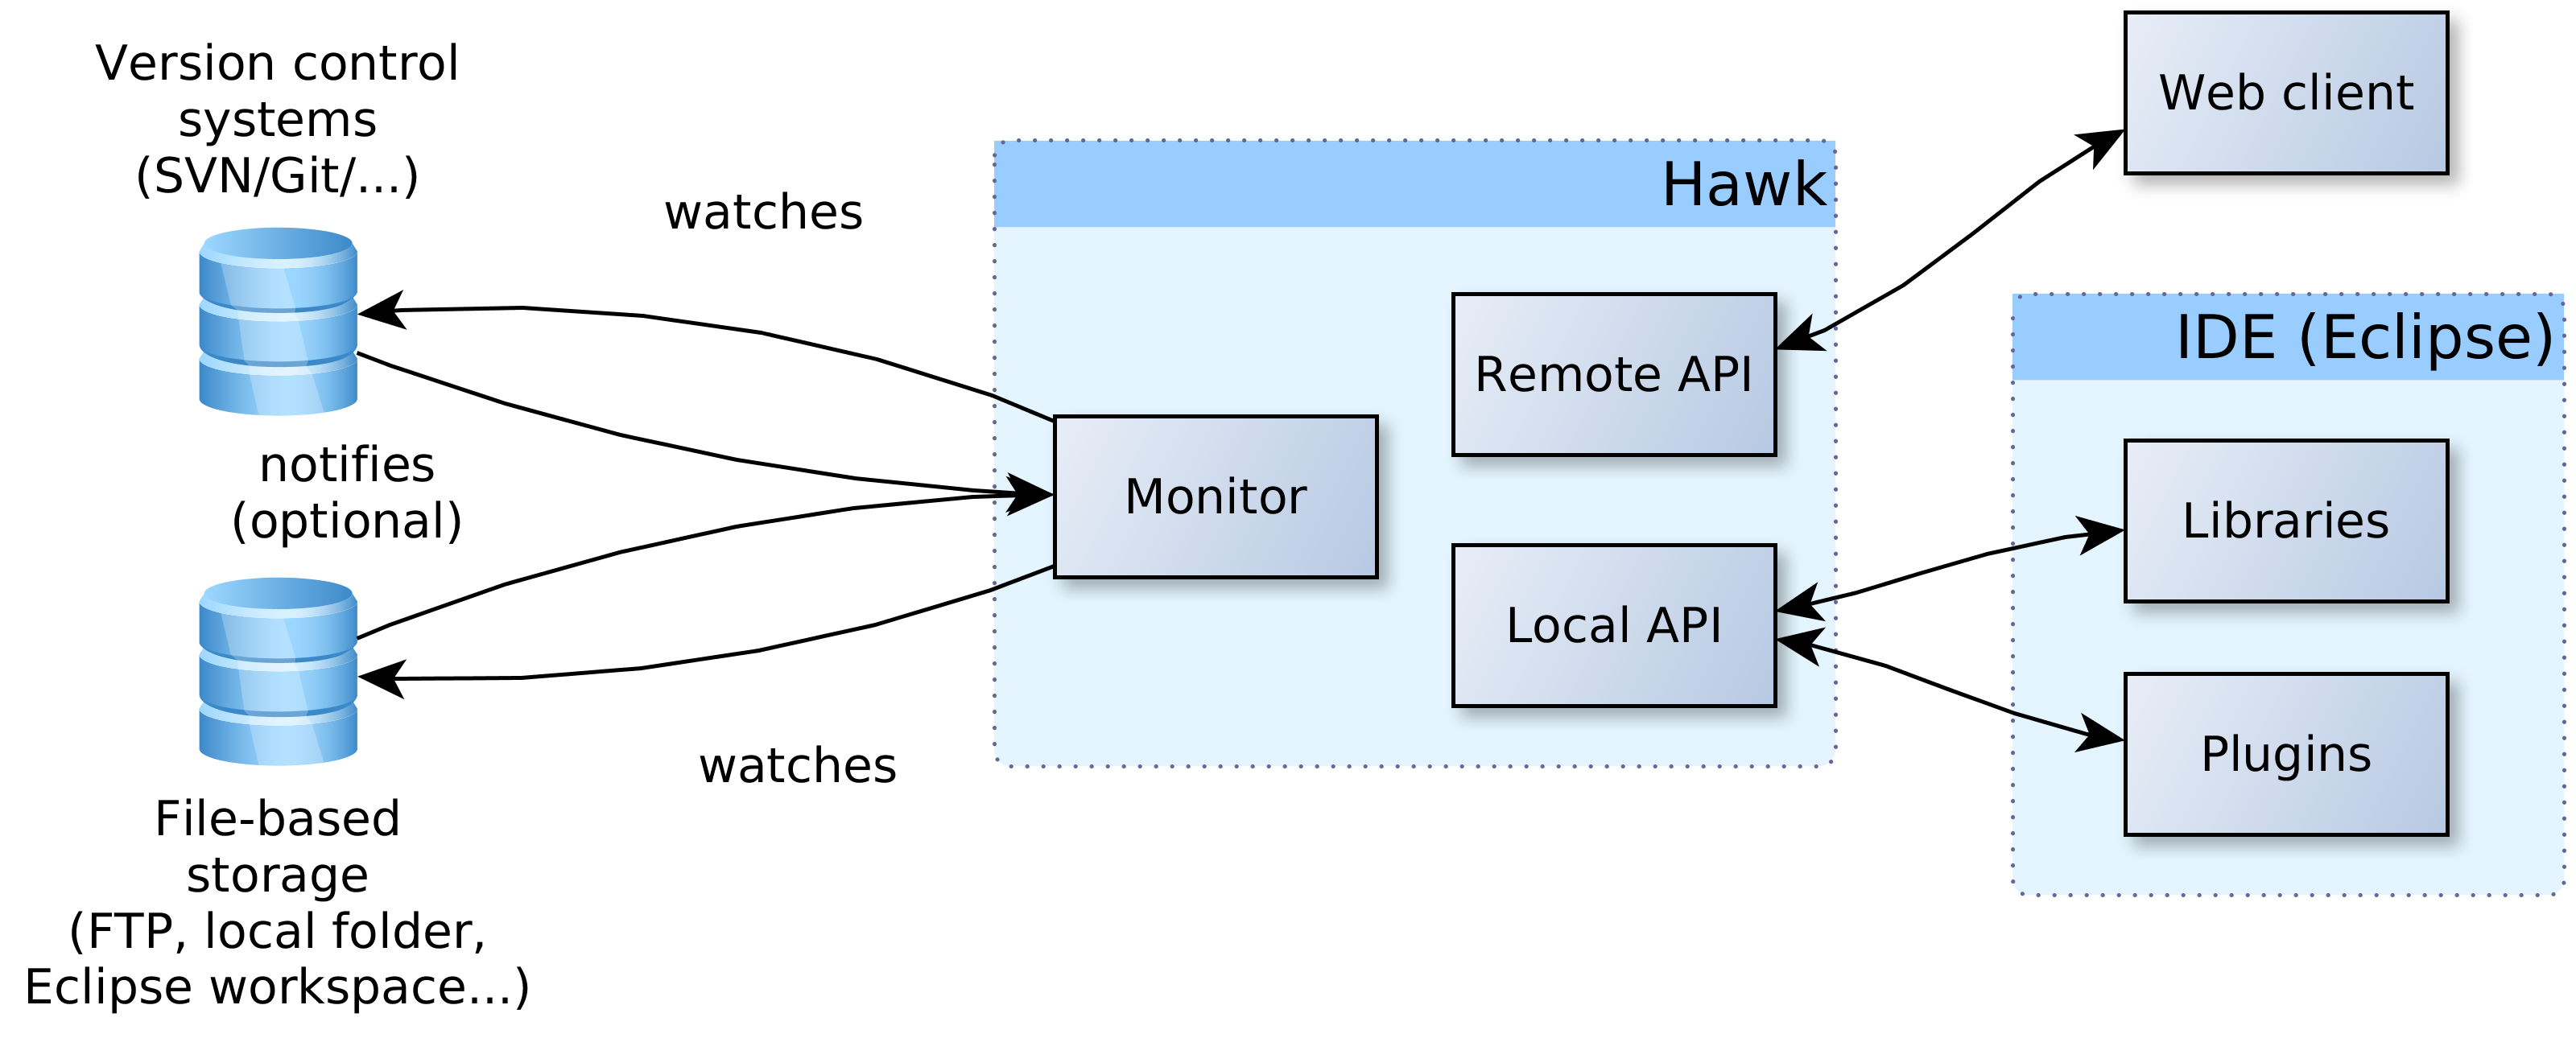
\includegraphics[width=\textwidth]{hawk-deployment}
  \end{center}

  \begin{itemize}
  \item Hawk can run as Eclipse plug-in, Java library, or network service
  \item We can have it watch over various types of locations:
    \begin{itemize}
    \item Version control systems (SVN/Git repositories)
    \item File stores (local folders, Eclipse workspaces, HTTP locations)
    \end{itemize}
  \end{itemize}

\end{frame}

\begin{frame}{Component-based architecture}
  \begin{center}
    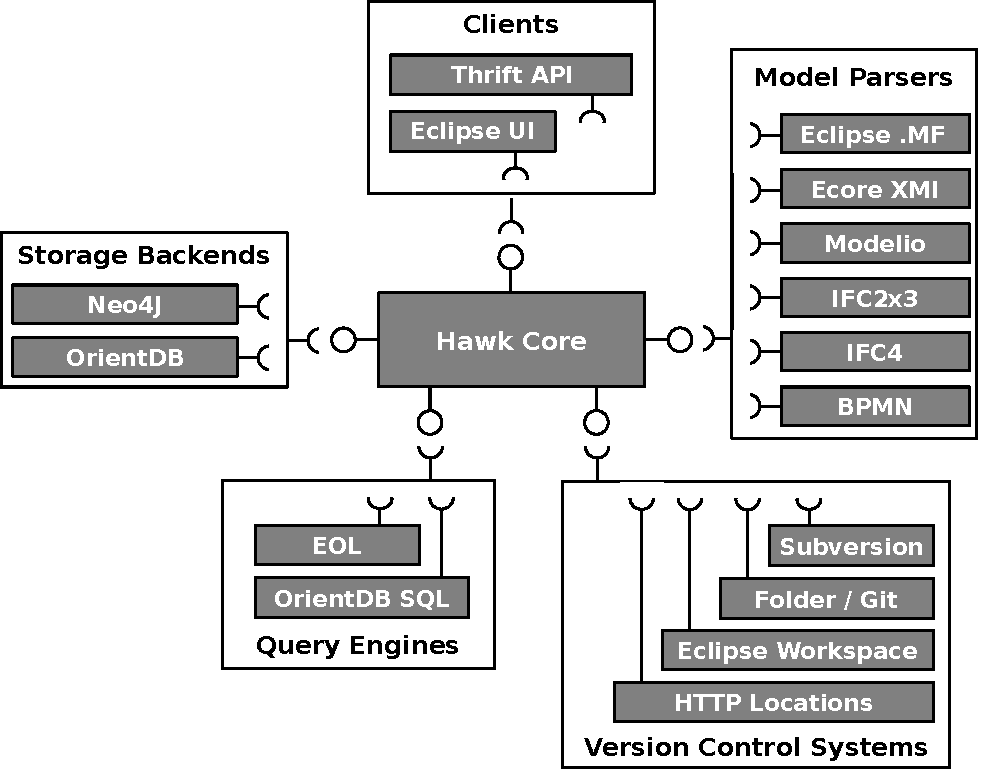
\includegraphics[width=.6\textwidth]{hawk-architecture}
  \end{center}

  \begin{itemize}
  \item Core: incremental graph updating + component interfaces
  \item Backends: Neo4j (fastest), OrientDB (multi-master), Greycat
  \item Clients: Eclipse GUI, cross-language Apache Thrift web services
  \item Query engines: Epsilon Object/Pattern Languages, OrientDB SQL
  \item Model parsers: EMF/Modelio models, Eclipse plug-in manifests...
  \end{itemize}
\end{frame}

\begin{frame}{Example for a library model}
  \centering
  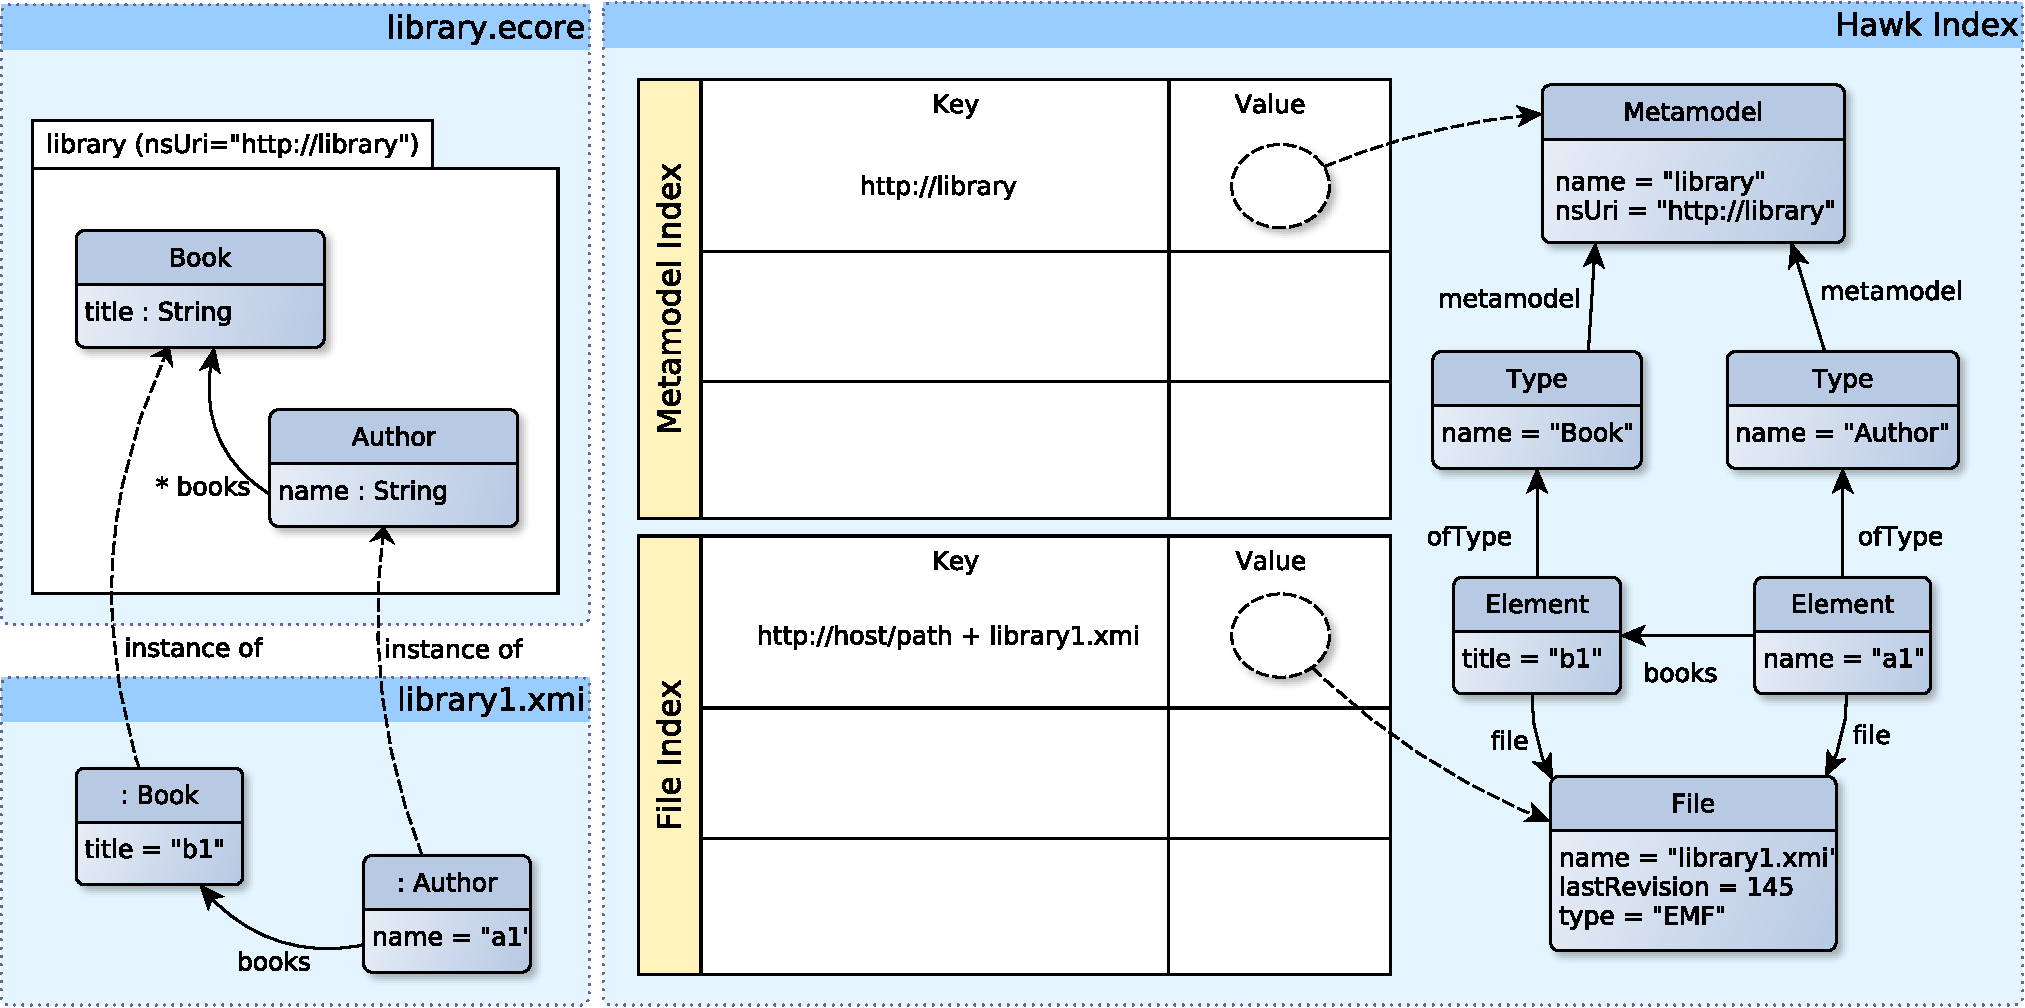
\includegraphics[width=\textwidth]{hawk-library-cropped}
  \begin{overprint}
    \onslide<1>
    \begin{tikzpicture}[remember picture,overlay]
      \draw[fill=white,fill opacity=0.8,draw=none]
      (page cs:-0.345,-0.4) rectangle (page cs:0.9,0.78);
    \end{tikzpicture}
    \begin{center}
      We go from these model files...
    \end{center}

    \onslide<2>
    \begin{tikzpicture}[remember picture,overlay]
      \draw[fill=white,fill opacity=0.8,draw=none]
        (page cs:-1.0,0.78) rectangle (page cs:-0.345,-0.4);
    \end{tikzpicture}
    \begin{center}
      ... to these NoSQL graphs.
    \end{center}

    \onslide<3>
    \begin{tikzpicture}[remember picture,overlay,every node/.style={draw=red,very thick},every edge/.style={draw=red,very thick,->}]
      %\printtikzpagegrid
      % \node[minimum width=2em,minimum height=.8em] (nbook) at (page cs:-.675,.405) {};
      % \node[minimum width=6.5em,minimum height=.9em] (nlibrary) at (page cs:-.65,.53) {};
      % \node[minimum width=2em,minimum height=.8em] (nauthor) at (page cs:-.515,.205) {};
      % \node[minimum width=2em,minimum height=.8em] (nbooki) at (page cs:-.71,-.19) {};
      % \node[minimum width=2em,minimum height=.8em] (nauthori) at (page cs:-.47,-.29) {};
      % \node[minimum width=3em,minimum height=.8em] (nmetamodel) at (page cs:.57,.57) {};
      % \node[minimum width=2em,minimum height=.8em] (nbookt) at (page cs:.44,.27) {};
      % \node[minimum width=2em,minimum height=.8em] (nauthort) at (page cs:.695,.27) {};
      % \node[minimum width=2em,minimum height=.8em] (nbooke) at (page cs:.435,.02) {};
      % \node[minimum width=2em,minimum height=.8em] (nauthore) at (page cs:.695,.02) {};
      % \node[minimum width=2em,minimum height=.8em] (nfile) at (page cs:.57,-.2) {};
      % \node[minimum width=6.5em,minimum height=.8em] (nmetamodelkey) at (page cs:-.062,.485) {};
      % \node[minimum width=6.5em,minimum height=.8em] (nfilekey) at (page cs:-.062,-.015) {};
      % \path
      %   (nlibrary) edge[out=0,in=180] (nmetamodel)
      %   (nbook) edge[out=0,in=180] (nbookt)
      %   (nauthor) edge[out=0,in=200] (nauthort);

      \draw[fill=white,fill opacity=0.8,draw=none]
        (page cs:-0.9,-.4) rectangle (page cs:-.35,.02);
      \draw[fill=white,fill opacity=0.8,draw=none]
        (page cs:-0.345,-.4) rectangle (page cs:0.34,0.78);
      \draw[fill=white,fill opacity=0.8,draw=none]
        (page cs:0.34,-.4) rectangle (page cs:0.85,0.15);
    \end{tikzpicture}
    \begin{itemize}
    \item Ecore packages $\rightarrow$ metamodel nodes
    \item Ecore classes $\rightarrow$ type nodes
    \end{itemize}

    \onslide<4>
    \begin{tikzpicture}[remember picture,overlay]
      \draw[fill=white,fill opacity=0.8,draw=none]
        (page cs:-.35,.02) rectangle (page cs:-0.9,.78);
      \draw[fill=white,fill opacity=0.8,draw=none]
        (page cs:-0.345,-0.4) rectangle (page cs:0.34,0.78);
      \draw[fill=white,fill opacity=0.8,draw=none]
        (page cs:0.85,0.15) rectangle (page cs:0.34,0.78);
    \end{tikzpicture}
    \begin{itemize}
    \item Physical files $\rightarrow$ file nodes
    \item Model elements $\rightarrow$ element nodes
    \end{itemize}

    \onslide<5>
    \begin{tikzpicture}[remember picture,overlay]
      \draw[fill=white,fill opacity=0.8,draw=none]
        (page cs:-.35,-.4) rectangle (page cs:-0.9,.78);
      \draw[fill=white,fill opacity=0.8,draw=none]
        (page cs:0.85,-.4) rectangle (page cs:0.34,0.78);
    \end{tikzpicture}
    \begin{itemize}
    \item MM index: package URI $\rightarrow$ metamodel node
    \item File index: file path $\rightarrow$ file node
    \item Users can define custom indices by attribute/expression
    \end{itemize}
  \end{overprint}
\end{frame}

\begin{frame}[standout]
  Hands-on time!

  Let's index a Java model and find singletons.
\end{frame}

\newcommand{\screenshot}[3]{
  \begin{frame}{#1}
    \begin{center}
      \includegraphics[width=\textwidth, height=.7\textheight, keepaspectratio]{#2}

      #3
    \end{center}
  \end{frame}
}

\screenshot{Preparing the workspace}{00-workspace}{
  Open Eclipse and import \file{tutorial.common} and \file{tutorial.hawk}.
}

\screenshot{Opening the main Hawk view}{01-open-view}{}

\screenshot{Adding a new Hawk index}{02-add}{
  Click on the ``Add'' button. We can keep as many different indices as we want
  within the same Eclipse installation.
}

\screenshot{Options, options!}{03-add-dialog}{
  There are many options here: we can use a local or a remote Hawk, we can
  choose the backend, and we can enable/disable plugins at will.
}

\screenshot{Options for the JDTAST models}{04-add-dialog-filled}{
  We will go with a local, Neo4j-based, EMF-focused index.
}

\screenshot{Index created}{05-created}{
  We have created an empty index. Time to configure it.
}

\screenshot{Configuring the index}{06-configure-button}{
  Let's click on the ``Configure'' button. This will open a new dialog.
}

\screenshot{Configure dialog}{06-configure-dialog}{
  The dialog is divided into tabs for managing metamodels, locations to index,
  and indexed/derived properties.
}

\screenshot{Adding metamodels}{07-add-mm-workspace}{
  Click on ``Add from workspace'' and select the Ecore, XMLTypes and
  JDTAST metamodels. These will be turned into Neo4j nodes and edges.
}

\screenshot{Added metamodels}{08-added-mm}{
  The metamodels have been registered: we can index models now.
}

\screenshot{Add locations}{09-add-locations}{
  Go to the ``Indexed Locations'' tab and click on ``Add''.
}

\screenshot{Adding a local folder}{10-localfolder}{
  We want to index the ``LocalFolder'' in the \file{tutorial.common/models/set1} folder.
}

\screenshot{Added local folder}{11-added-folder}{
  Wait a bit, watching the ``Status'' column, and the models will be indexed.
  Once it's done, the index is ready to be queried.
}

\screenshot{Query button}{12-query-button}{
  Click on the ``Query'' button.
}

\screenshot{Query dialog: main tab}{13-query-dialog}{
  The ``Query'' dialog is quite involved: let's go bit by bit.

  The main page allows us to enter the query by hand, from a file or from the
  current editor, run/stop/reset it, and request manual syncs.
}

\screenshot{Query dialog: path-based scope}{14-path-scope}{
  We could optionally limit the scope of the query to specific repositories and/or files.
  This can be useful when querying large collections of models.

  Patterns are essentially glob-style: e.g. \file{folder/f*.xmi}.
}

\screenshot{Query dialog: subtree-based scope}{15-subtree-scope}{
  Another option is to limit scope to the objects contained within a certain top-level
  file. This can be useful when querying hierarchically fragmented models (e.g. those
  created with EMF-Splitter by Antonio Garmendia).
}

\screenshot{Query dialog: default namespaces}{16-default-ns}{
  In some cases, ``Type.all'' might be ambiguous as we may have multiple types
  with the same unqualified name. Here we can specify which metamodel URIs should
  take precedence.
}

\screenshot{Query dialog: traversal scoping}{17-traversal-scoping}{
  When following references from an object, we may want to ignore the ones that leave
  the path-/subtree-based scope that we defined before.
}

\screenshot{Query dialog: entering a query}{18-query-entered}{
  Let's go back to the main tab and enter a simple query about the number of instances
  of a class. Click on ``Run Query'', which will temporarily change to ``Stop Query''.
}

\screenshot{Query dialog: query executed}{19-query-executed}{
  The query finished running, and here we have the results.

  Now that we know the basic use of Hawk, let's move to the more advanced features.
}

\begin{frame}[fragile]{Indexed attributes}
  \begin{block}{Finding a type by its name (\file{findByName.eol})}
    \lstinputlisting[language=EOL]{listings/set0-findByName.eol}
  \end{block}

  \begin{block}{This normally involves...}
    \begin{enumerate}
    \item Iterating over all types
    \item Following the ``name'' reference
    \item Comparing the name
    \end{enumerate}
  \end{block}

  \begin{alertblock}{Replace with a lookup (\file{findByName-indexed.eol})}
    \vspace{.3em}
    We only need to tell it to index ``SimpleName.identifier'':
    \lstinputlisting[language=EOL]{listings/set0-findByName-indexed.eol}
  \end{alertblock}
\end{frame}

\screenshot{Indexed attributes tab}{22-iattr-tab}{
  Go back to the ``Configure'' tab and select the ``Indexed Attributes''
  tab. Click on ``Add'', and a new dialog should pop up.
}

\screenshot{Options for the indexed attribute}{23-iattr-dialog}{
  Use the combo boxes to pick the metamodel, type and attribute
  shown above. Click on ``Add''.
}

\begin{frame}[fragile]{Derived attributes}
  \begin{block}{Original query for finding singletons (\file{singletons.eol})}
    \lstinputlisting[language=EOL]{listings/singletons.eol}
  \end{block}

  \begin{block}{Can we do it faster?}
    \begin{itemize}
    \item Checking if a method is public or static requires traversing
      references
    \item Same goes for checking if it returns an instance of itself
    \item In Hawk, \alert{we can precompute this}
    \item When files change, only the affected values are recomputed
    \end{itemize}
  \end{block}
\end{frame}

\begin{frame}[fragile]{Use of derived attributes as precomputed values}

  \begin{block}{Original query (\file{singletons.eol})}
    \lstinputlisting[language=EOL]{listings/singletons.eol}
  \end{block}

  \begin{block}{Changed for MethodDeclaration derived attributes (\file{singletons-dmethods.eol})}
    \lstinputlisting[language=EOL,firstline=13]{listings/singletons-dmethods.eol}
  \end{block}
\end{frame}

\screenshot{Derived attributes tab}{25-dattr-tb}{
  Now we move to the ``Derived Attributes'' tab of the configure dialog.
}

\screenshot{Options for one of the derived attributes}{26-dattr-dialog}{
  For the first derived attribute, fill in the form as above. You can load the
  EOL code straight from the workspace --- no need to copy and paste!
}

\begin{frame}{Derived attributes are also indexed}
  \begin{block}{Revised query (\file{singletons-dmethods.eol})}
    \lstinputlisting[language=EOL,firstline=13]{listings/singletons-dmethods.eol}
  \end{block}

  \begin{block}{Can we do it faster?}
    \begin{itemize}
    \item Right now, we need to go through \emph{all} type declarations and then
      filter by methods
    \item What if we go from the methods to the types instead?
    \item In Hawk, \alert{top-level selects can replace iteration with lookups
      when using derived attributes}
    \end{itemize}
  \end{block}
\end{frame}

\begin{frame}{Use of derived attributes as index keys}

  \begin{block}{Previous query (\file{singletons-dmethods.eol})}
    \lstinputlisting[language=EOL,firstline=13]{listings/singletons-dmethods.eol}
  \end{block}

  \begin{block}{Revised to use index, with derived attrs. at top level (\file{singletons-dmethodsindexed.eol})}
    \lstinputlisting[language=EOL]{listings/singletons-dmethodsindexed.eol}
  \end{block}

\end{frame}

\begin{frame}[fragile]{Flagging singletons directly}
  \begin{block}{Previous query (\file{singletons-dmethodsindexed.eol})}
    \lstinputlisting[language=EOL]{listings/singletons-dmethodsindexed.eol}
  \end{block}

  \begin{block}{Can we do it faster?}
    \begin{itemize}
    \item We could just flag types that are singletons
    \item This derived attribute might be less reusable, however
    \end{itemize}
  \end{block}
\end{frame}

\begin{frame}[fragile]{Final query for finding singletons}
  \begin{block}{Previous query (\file{singletons-dmethodsindexed.eol})}
    \lstinputlisting[language=EOL]{listings/singletons-dmethodsindexed.eol}
  \end{block}

  \begin{block}{Final query (\file{singletons-dtypes.eol})}
    \lstinputlisting[language=EOL,firstline=12]{listings/singletons-dtypes.eol}
  \end{block}
\end{frame}

\begin{frame}[standout]
  Hands-on time!

  This time, we will show how to use indexed and derived attributes.
\end{frame}

\begin{frame}[fragile]{Derived edges}
  \begin{block}{Toy example: Person metamodel}
    \begin{itemize}
    \item Person metamodel, with ``parents'' references.
    \item We want to be able to quickly find siblings, grandparents,
      uncles/aunts, cousins, second-cousins, ancestors...
    \item We can precompute this in Hawk with \alert{derived edges}
    \end{itemize}
  \end{block}

  \begin{block}{Derivation logic for ``grandparents'' (\file{Person\_grandparents.eol})}
    \vspace{.3em}
    We need a flat list and not a list of lists, so we use ``flatten'':
    \begin{lstlisting}[language=EOL]
      return self.parents.parents.flatten;
    \end{lstlisting}
  \end{block}

  \begin{block}{Derivation logic for ``siblings'' (\file{Person\_siblings.eol})}
    \vspace{.3em}
    We can travel references in reverse with ``revRefNav\_name'':

    \begin{lstlisting}[language=EOL]
      return self.parents.revRefNav_parents.flatten.excluding(self);
    \end{lstlisting}
  \end{block}

\end{frame}

\begin{frame}[standout]
  Last hands-on slot for Hawk.

  We will show derived edges this time.
\end{frame}

\begin{frame}{Hawk: integration into SOFTEAM Constellation~\cite{hawkmodelio_2016}}

  \centering
  \begin{columns}
    \column{.5\textwidth}
    \begin{center}
  \resizebox{\columnwidth}{!}{
    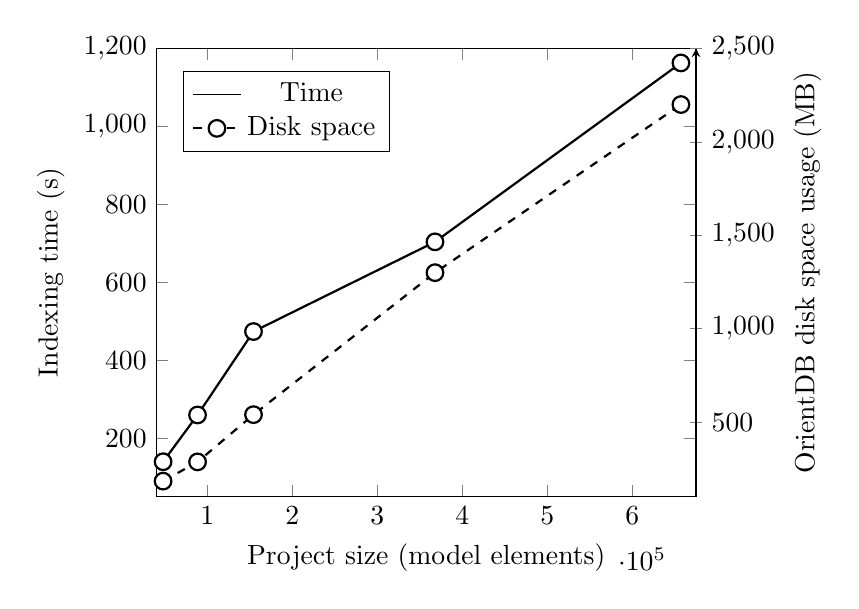
\begin{tikzpicture}
      \begin{axis}[
        xlabel={Project size (model elements)},
        ylabel={Indexing time (s)},
        xmin=40000,xmax=675000,
        ymin=50,ymax=1200
        ]
        \addplot+[black,thick,mark options={solid,mark size=3,fill=white}] coordinates {
          (47891, 140)
          (88451, 260)
          (154281, 474)
          (367840, 704)
          (657228, 1163)
        }; \label{Hplot}
      \end{axis}
      \begin{axis}[
        axis x line=none,
        axis y line=right,
        ylabel={OrientDB disk space usage (MB)},
        xmin=40000,xmax=675000,
        ymin=100,ymax=2500,
        legend style={at={(0.05,0.95)},anchor=north west}
        ]
        \addlegendimage{/pgfplots/refstyle=Hplot}\addlegendentry{Time}
        \addplot+[black,thick,dashed,mark options={solid,mark size=3,fill=white}] coordinates {
          (47891, 184)
          (88451, 287)
          (154281, 540)
          (367840, 1300)
          (657228, 2200)
        }; \addlegendentry{Disk space}
      \end{axis}
    \end{tikzpicture}
  }
  \textbf{Indexing times and index sizes (OrientDB backend)}
\end{center}


    \column{.4\textwidth}
    \begin{center}
  \resizebox{\columnwidth}{!}{
    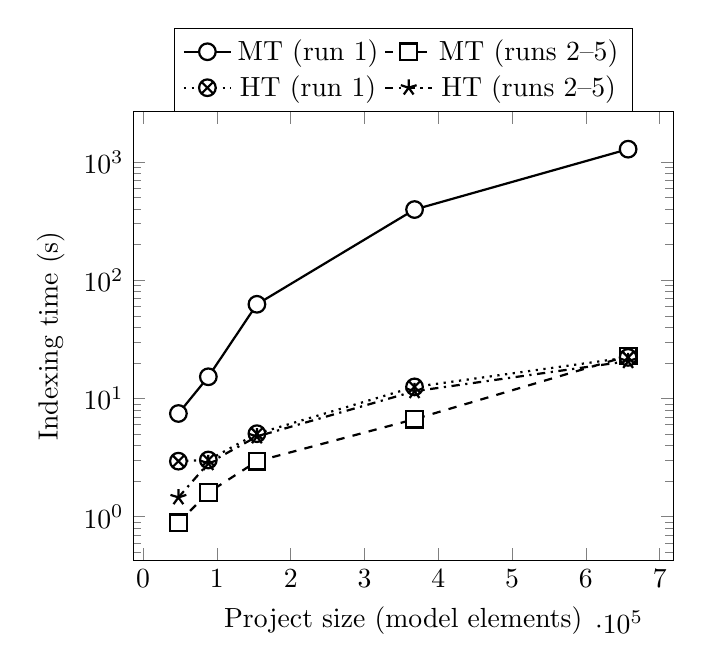
\begin{tikzpicture}
      \begin{semilogyaxis}[
        xlabel={Project size (model elements)},
        ylabel={Indexing time (s)},
        legend entries={
          {MT (run 1)},
          {MT (runs 2--5)},
          {HT (run 1)},
          {HT (runs 2--5)}
        },
        legend style={
          legend columns=2,
          at={(0.5,1)},
          anchor=south,
        },
        mark options={solid,mark size=3},
        ]
        \addplot+[black,thick,mark options={solid,mark size=3,fill=white}] coordinates {
          (47891, 7.465)
          (88451, 15.260)
          (154281, 62.550)
          (367840, 395.659)
          (657228, 1281.042)
        };
        \addplot+[black,thick,dashed,mark options={solid,mark size=3,fill=white}] coordinates {
          (47891, 0.890)
          (88451, 1.604)
          (154281, 2.944)
          (367840, 6.682)
          (657228, 22.891)
        };
        \addplot+[black,thick,dotted,mark options={solid,mark size=3,fill=white}] coordinates {
          (47891, 2.951)
          (88451, 3.019)
          (154281, 5.039)
          (367840, 12.531)
          (657228, 22.247)
        };
        \addplot+[black,thick,dashdotted] coordinates {
          (47891, 1.457)
          (88451, 2.834)
          (154281, 4.771)
          (367840, 11.510)
          (657228, 20.661)
        };
      \end{semilogyaxis}
    \end{tikzpicture}
  }
  \textbf{Code generation times: Modelio (MT), Hawk (HT)}
\end{center}

  \end{columns}

  \begin{itemize}
  \item Constellation: collaboration platform over Modelio models
  \item SOFTEAM needed search, couldn't change persistence
  \item Integrated Hawk as a library: initial indexing cost quickly paid off
  \end{itemize}
\end{frame}

\begin{frame}{Stress-testing remote query APIs~\cite{sosym-stress-2017}}

  \begin{center}
    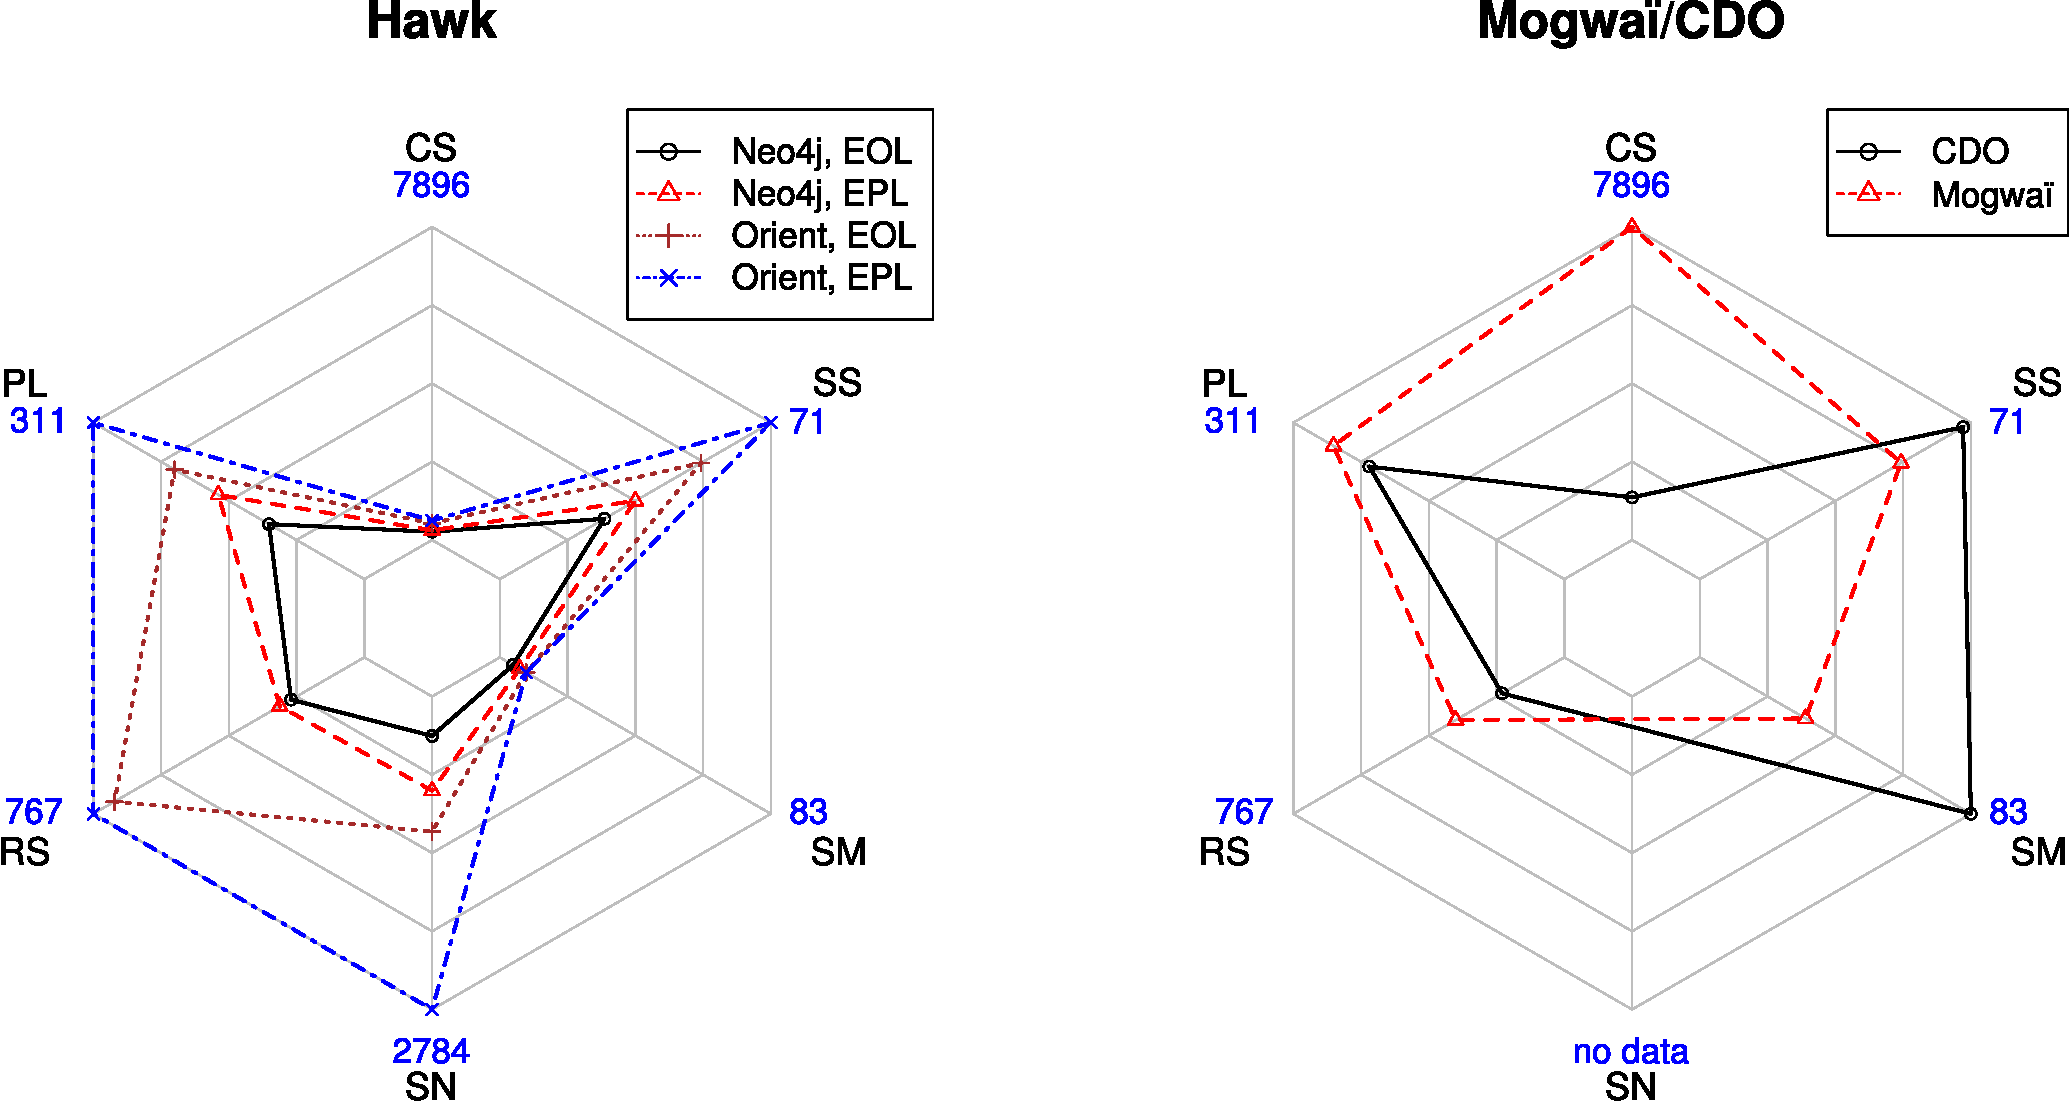
\includegraphics[width=\textwidth]{rq3-comparison-tb}
  \end{center}

  \begin{itemize}
  \item Included CDO, Hawk, Mogwaï and ranged 1--64 clients
  \item Reverse reference navigation was crucial in having the
    SN Train Benchmark~\cite{trainbenchmark} query run quickly
  \end{itemize}

\end{frame}

\begin{frame}[fragile]{Time-aware queries in Hawk over versioned models~\cite{hawk-mrt2018}}

  \begin{lstlisting}[frame=tb,language=EOL,escapechar=@,basicstyle=\footnotesize]
var rs = RewardTableRow@\textcolor{red}{.latest}@.all.collect(row | row.getRewardShifts()).flatten();
return Sequence { rs.min(), rs.max(), rs.average() };

operation RewardTableRow getRewardShifts(): Sequence {
  var v = self@\textcolor{red}{.versions}@;
  if (v.size <= 1) { return Sequence {}; }
  else { return v.subList(0, v.size - 1).collect(v | v.value - v@\textcolor{red}{.prev}@.value); }
}
operation Sequence average() { return self.sum() / self.size(); }
  \end{lstlisting}

  \begin{itemize}
  \item Extended Hawk with Greycat temporal graph support and time-aware query
    engine / updater components
  \item Can index entire Subversion-based history of a model, and ask things
    about its history through a new set of time-aware primitives
  \item Above query is finding descriptive stats for reward table shifts in a
    models@run.time system
  \item \alert{Presenting this work at 14:00 (MRT'18) --- hope to see you there!}
  \end{itemize}

\end{frame}

\begin{frame}{Hawk: project website}
  \begin{center}
    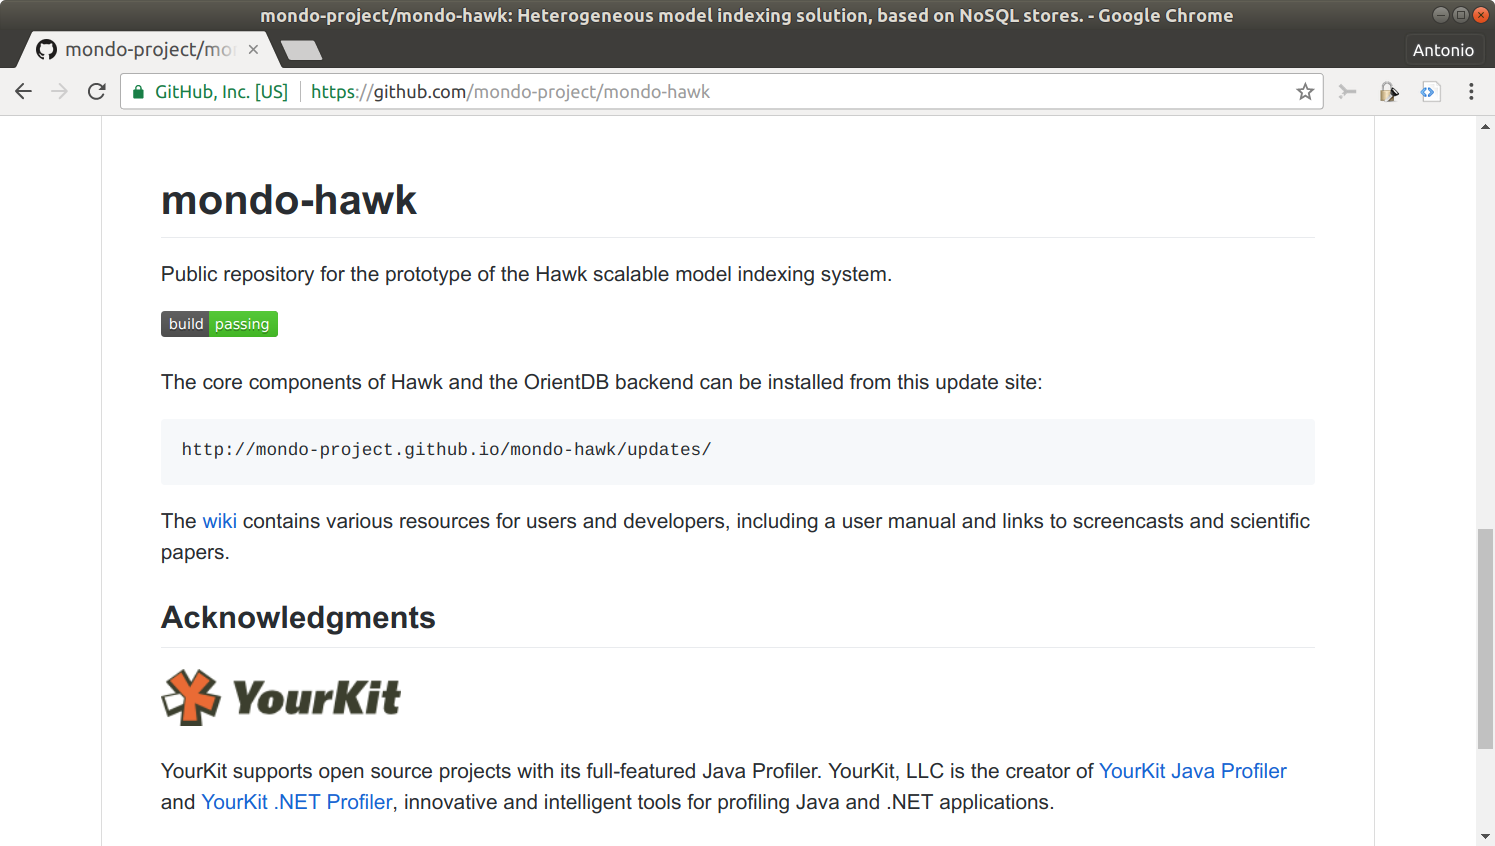
\includegraphics[width=\textwidth]{hawk-github}
  \end{center}

  \begin{itemize}
  \item \url{https://github.com/mondo-project/mondo-hawk}
  \item Recently accepted as Eclipse Incubator project (moving soon!)
  \end{itemize}
\end{frame}

\begin{frame}{Hawk: summing up}

  \begin{block}{So far...}
    \begin{itemize}
    \item Hawk is good for indexing an existing collection of model files
    \item You can efficiently answer queries from the index
    \item Indexed/derived features can be used to speed up queries
    \end{itemize}
  \end{block}

  \begin{block}{Ideas in the roadmap}
    \begin{itemize}
    \item Extensible UI, covering differences in options for components
    % Folding Space immediately asked about horizontal scaling, interestingly
    \item Horizontal scaling (a flock of Hawks?)
    \item Web UI based on Thrift API
    \item More backends! (Triple stores? Neo4j 3.x? MapDB?)
    \item Better Git connector (JGit-based)
    \item Extending EOL with Linear Temporal Logic
    \item Visualizations based on time-aware queries
    \end{itemize}

    Feedback and contributions are welcome!
  \end{block}

\end{frame}

\pgfset{/metropolis/inner/sectionpage/.cd, none}
\section{NeoEMF}

\section{Mogwa\"i}

\section{Wrap-up}

\begin{frame}[allowframebreaks]{References}

  \bibliography{../bibliography}
  \bibliographystyle{alpha}

\end{frame}

\end{document}
